\section*{Absorberande randvillkor}
%Ett numeriskt experiment i denna rapport går ut på att försöka implementera en absorberande rand till en domän [0,L] i en dimension. 

För att kontrollera det absorberande randvillkorets \eqref{eq:abc} realism görs följande numeriska experiment. Givet en domän [0,L] med randvillkoret \eqref{eq:abc} vid $x = 0$ och $x = L$ mäts vågens energi före och efter reflektion mot randen. Energin ska vara proportionell mot vågens amplitud i kvadrat, om vi halverar amplituden vid reflektion, $\alpha = 0.5$, så borde energin reduceras till en fjärdedel. I figur 2 presenteras resultatet av simuleringen med $\alpha = 0.5$. Simuleringen görs över en hel period T, alltså från initialläget tills vågen reflekterats och är tillbaka i startpositionen.\\*
\newline
\begin{minipage}{\linewidth}
\begin{tabular}{llll}
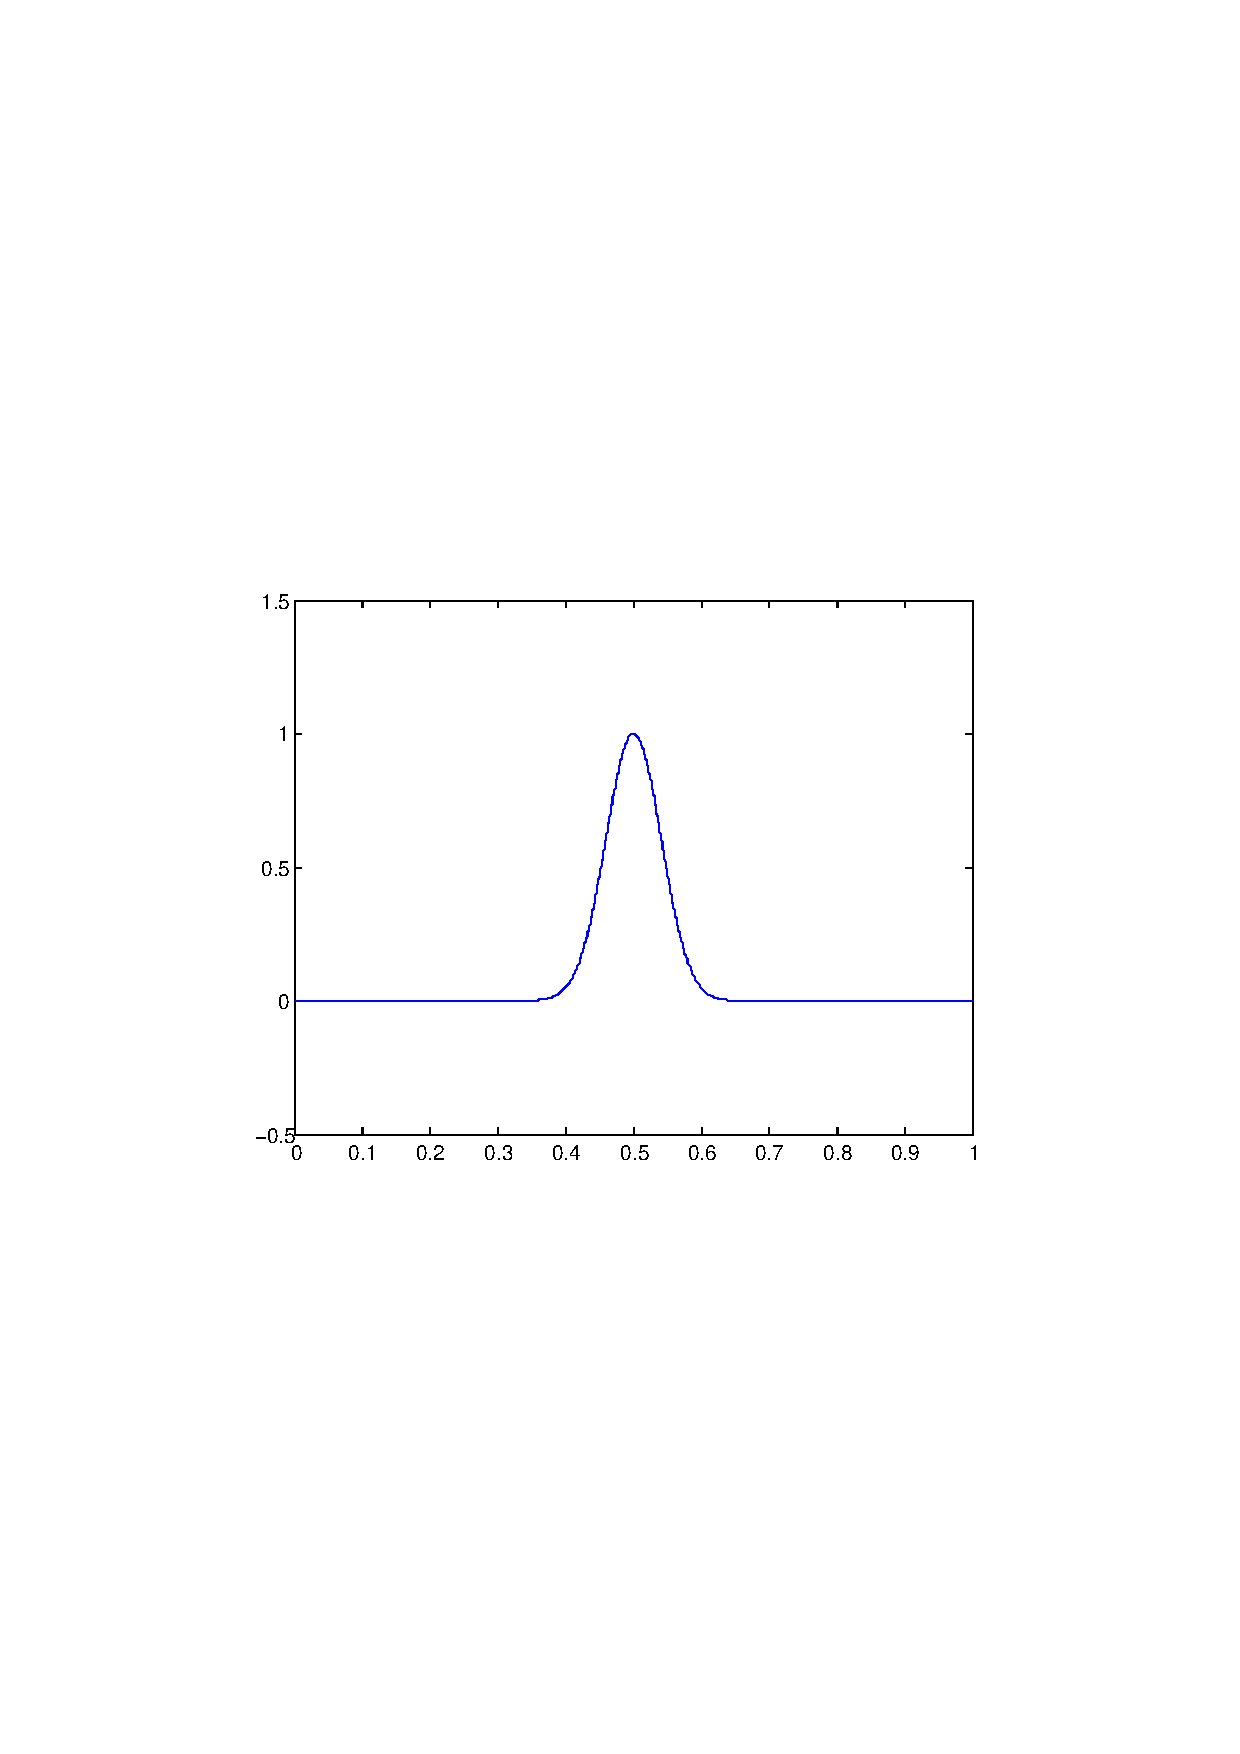
\includegraphics[trim = 5cm 10cm 4cm 10cm, width=.24\linewidth]{abc1.pdf} &
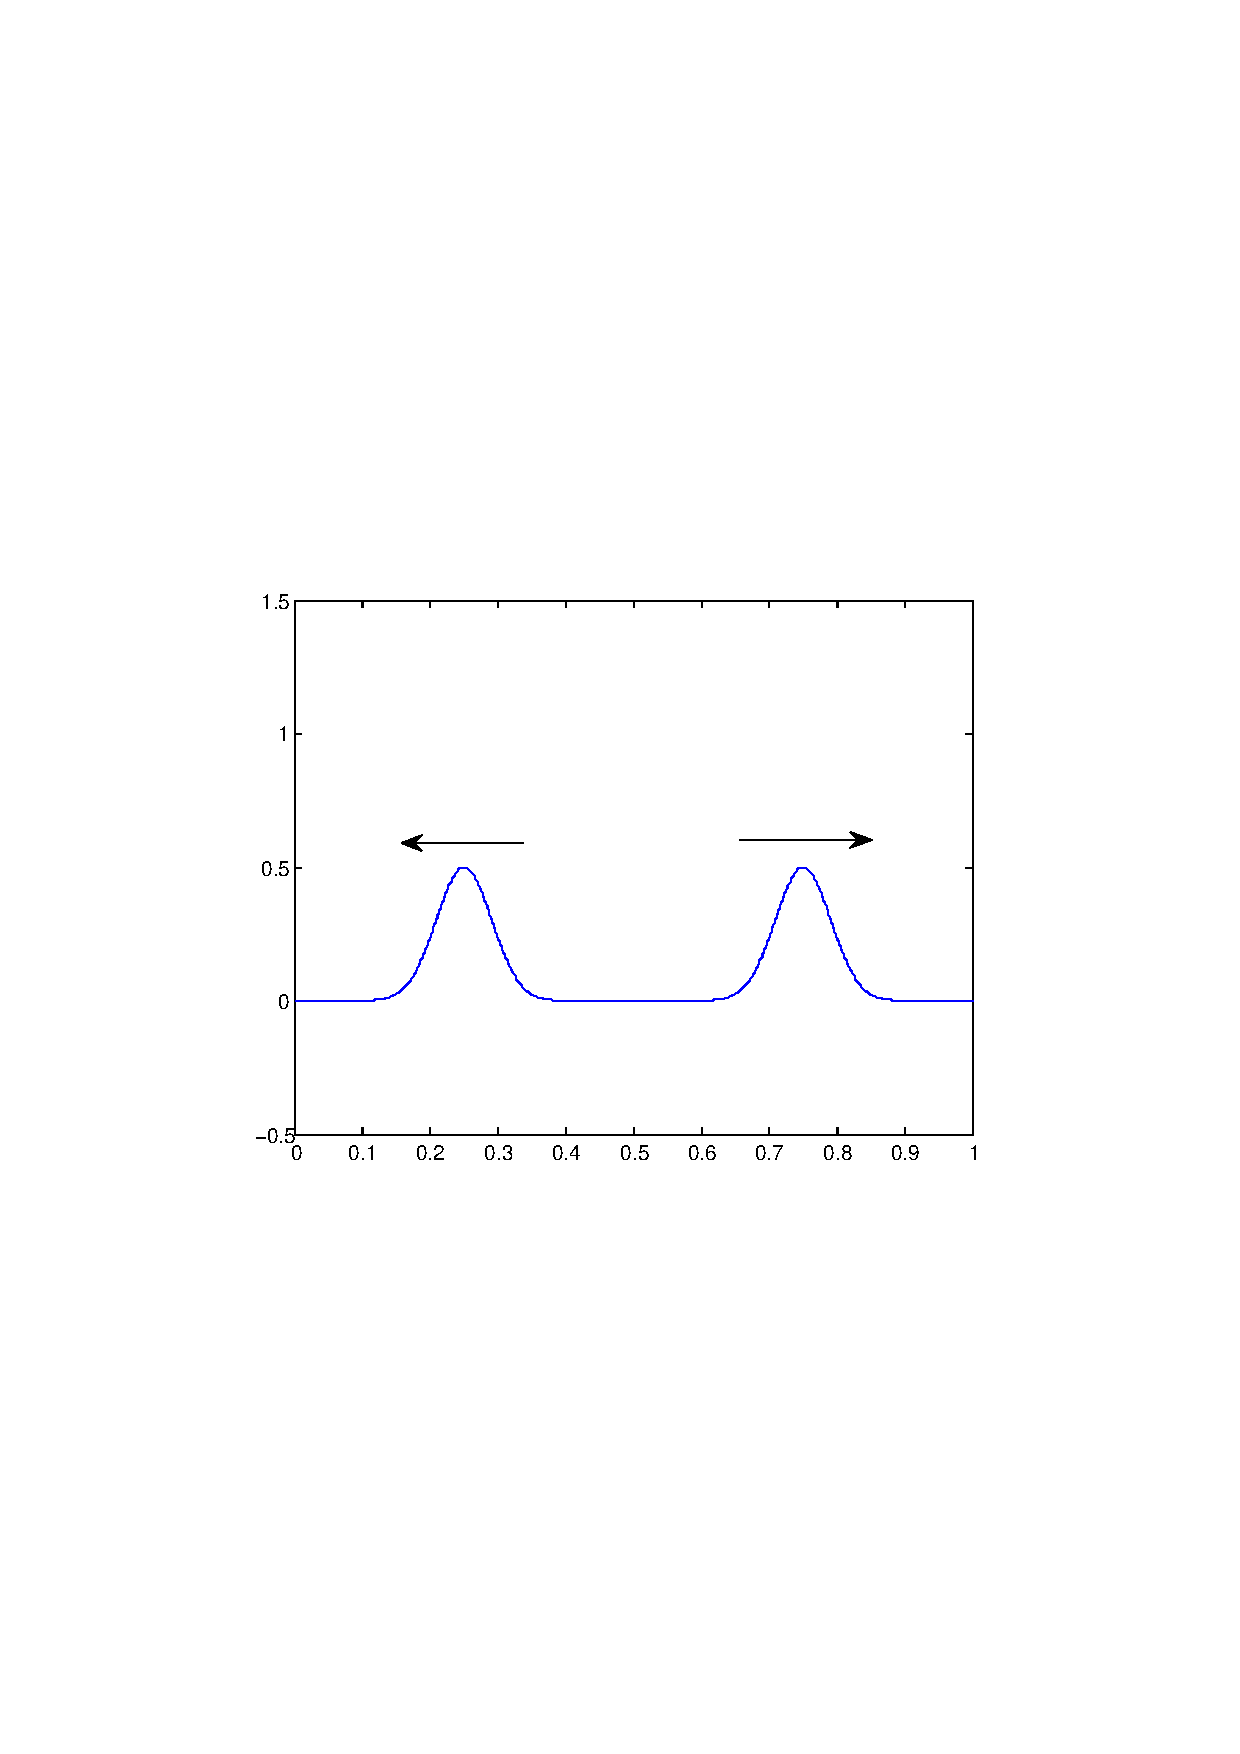
\includegraphics[trim = 5cm 10cm 4cm 10cm, width=.24\linewidth]{abc2.pdf} &
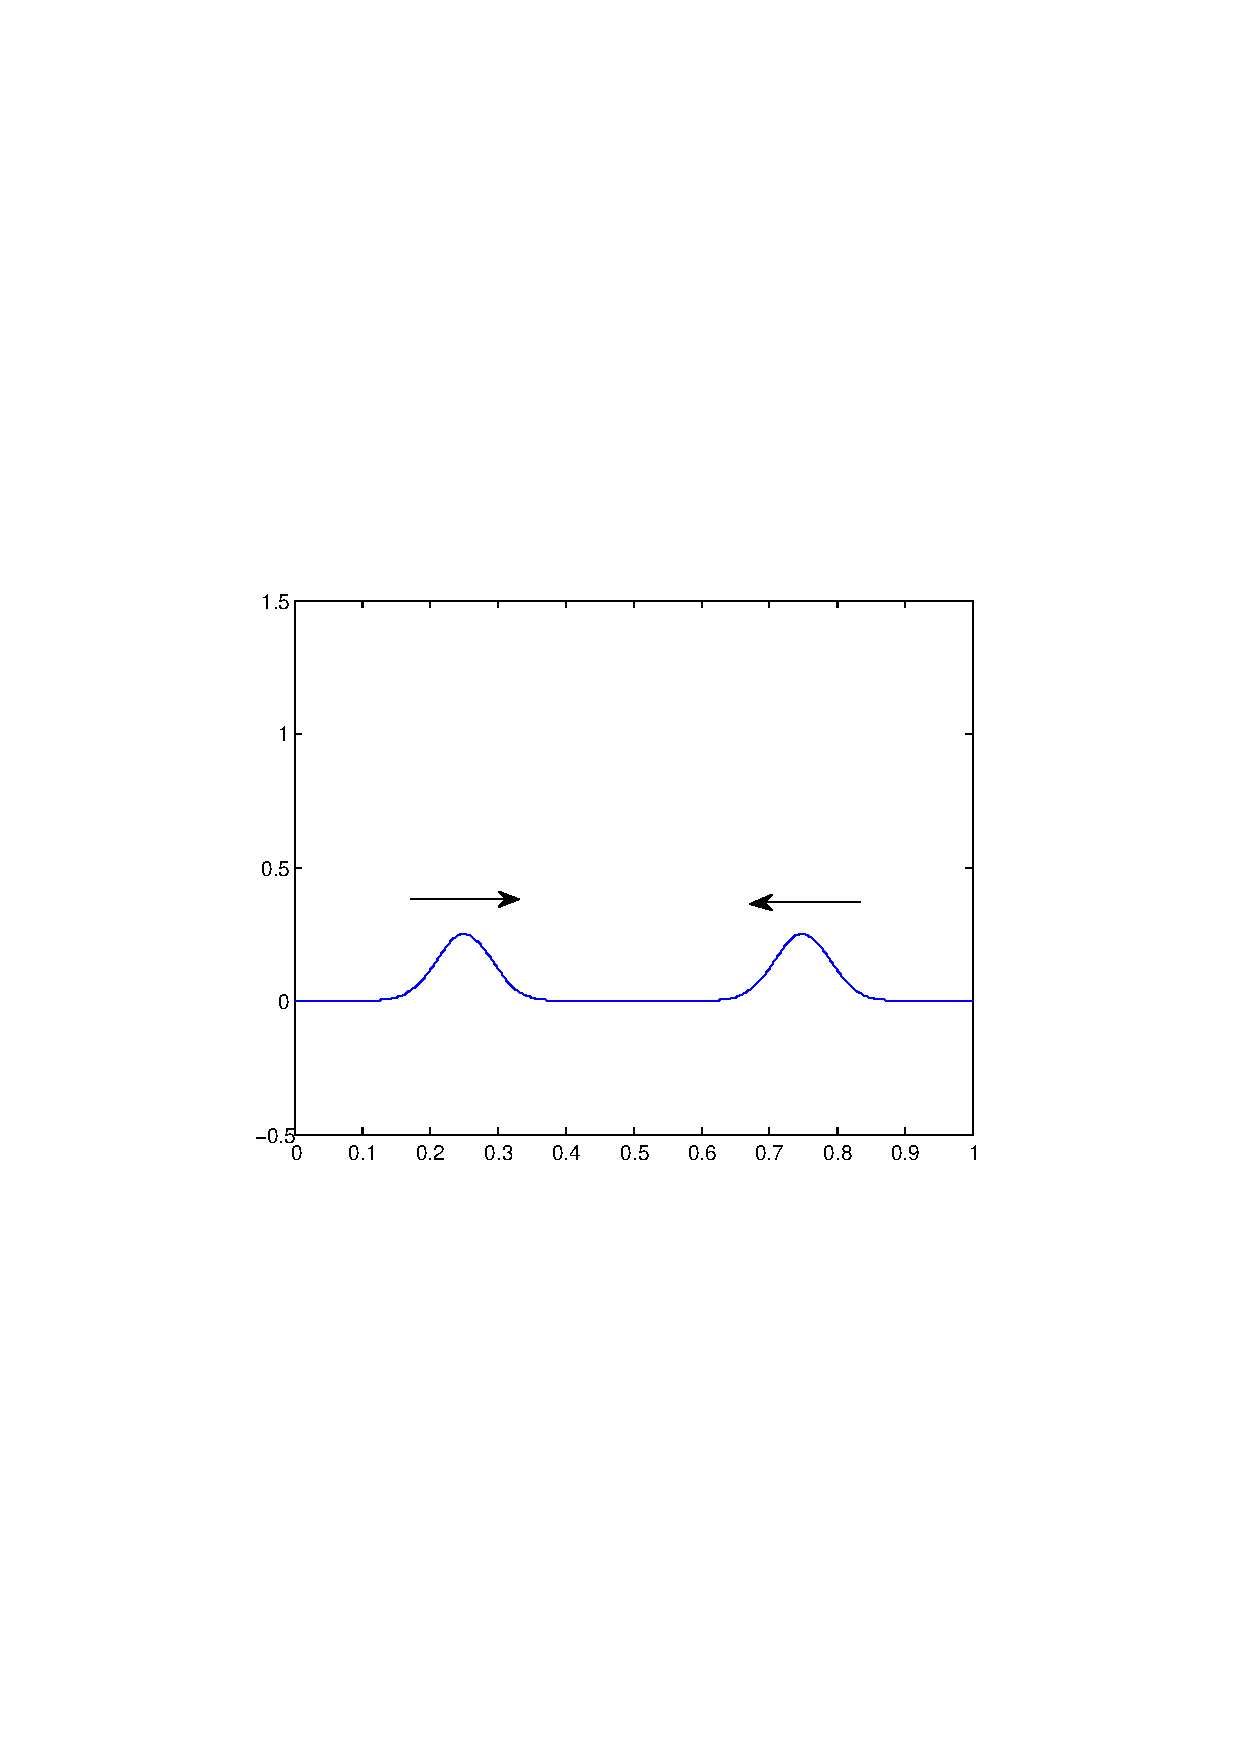
\includegraphics[trim = 5cm 10cm 4cm 10cm, width=.24\linewidth]{abc3.pdf} &
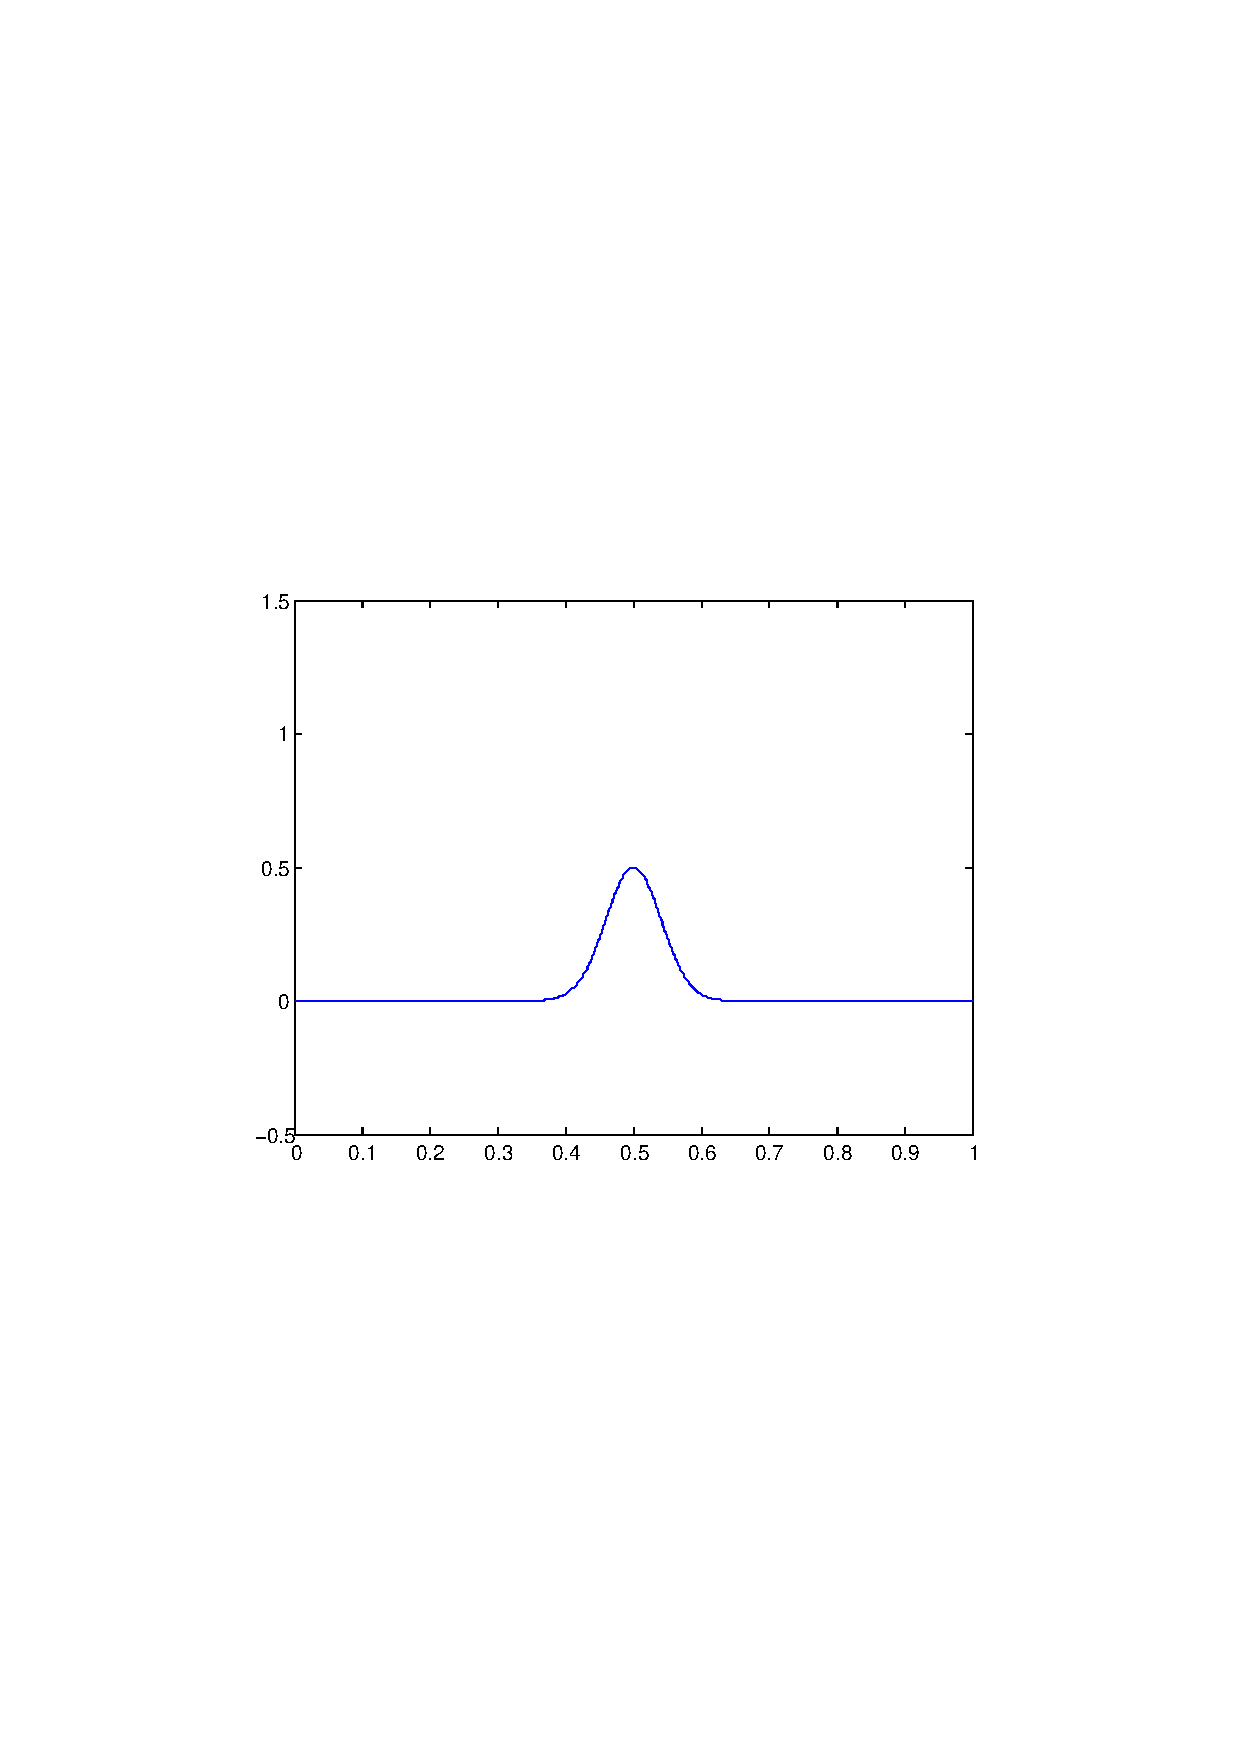
\includegraphics[trim = 5cm 10cm 4cm 10cm, width=.24\linewidth]{abc4.pdf}
\end{tabular}
\begin{center}
\caption{Figur 2. Från vänster ser vi vågen vid $t = 0$, $t = 0.25 T$, $t = 0.75 T$ och $t = T$.}\\*
\end{center}
\end{minipage}
\newline
\newline
Vågens energi mäts med en energiintegral härledd för Neumannvillkor. Denna ger ett inkorrekt resultat när vågen är nära randen, därför hämtas mätvärden när vågen helt lämnat randen. I tabell 1 kan det läsas av att medan amplituden har halverats så har energin minskat med en faktor fyra.\\*

\begin{minipage}{\linewidth}
	\begin{center}
    \begin{tabular}{| l | l | l | l |}
    \hline
    Tid & 0.25T &  0.75T \\ \hline
    Amplitud & 0.5 & 0.25 \\ \hline
    Energi & 10.8535 & 2.7136 \\ \hline
    \end{tabular}
    \end{center}
    \newline
    \begin{center}
    \caption{Tabell 1. Vågens amplitud och energi före och efter reflektion.}
    \end{center}
\end{minipage}

